\section{ Filler lecture:Volcanism and Planetary Interiors }\label{sec:q2}    

\subsection*{a)}
A mid-ocean ridge is the border between two oceanic plates that are moving away from each other. From the local thinning of the plates, and eventually the gap between the plates, matter from below the crust can seep upwards, until it solidifies on the ocean floor, forming long, elevated ridges, as seen in the left figure. In the right figure, there is an active continental margin. It is a continental margin, the boundary between a continental plate and an oceanic plate, where active volcanism occurs. Matter from the ocean floor is transported down along with the oceanic plate, and as it travels down, heats up and melts. This causes the molten material to rise upward and manifest in a volcanically active mountain ridge, also known as subduction volcanism. 
\begin{figure}[H]
    \centering
    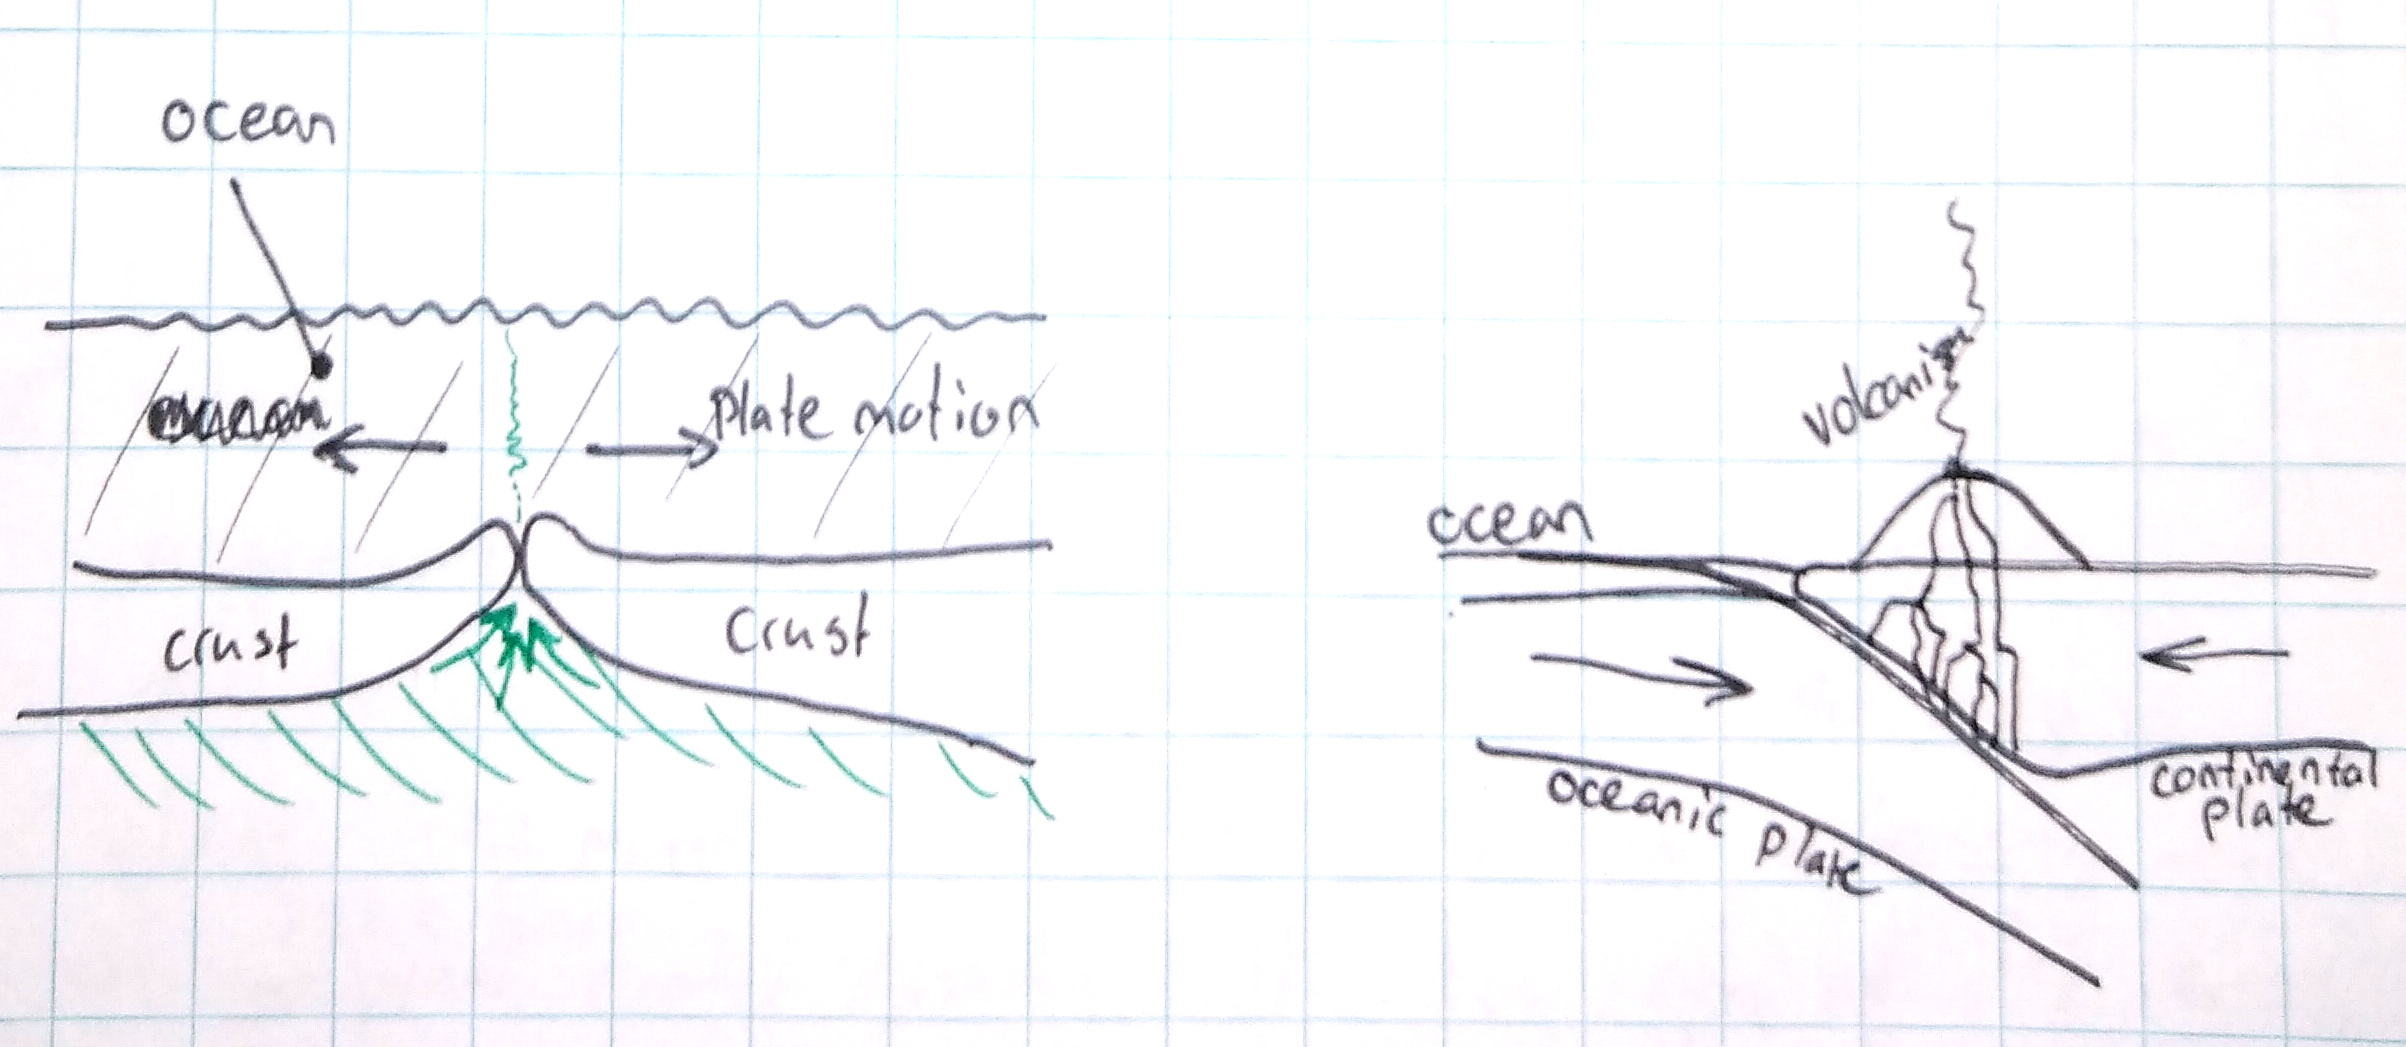
\includegraphics[width=0.8\textwidth]{figures/2b.jpg}
    %\caption{Caption}
    \label{fig:my_label2}
\end{figure}

\subsection*{b)}
The three types of volcanism that occur on Earth are:
\begin{enumerate}
    \item Mid-ocean ridge volcanism - Between two ocean plates that move apart.
    \item Subduction zone volcanism - Between an oceanic plate diving underneath a continental plate
    \item Hotspot volcanism - Most notable examples on Earth occur in ocean, caused by a local hotspot (plume) in the mantle rising upward and pushing hot material through the crust. The plates may move slowly over-top the hotspots, creating ridges on the ocean floor, or even islands (e.g. Hawaii).
\end{enumerate}

\subsection*{c)}
Cryovolcanism is a type of volcanism where instead of molten rock and metal, fluids such as water or methane, are expelled. This type of volcanism occurs under significantly lower temperatures too, hence the name. Cryovolcanism is most often encountered on icy moons, such as Europa, Enceladus, and Triton.

\subsection*{d)}
\begin{enumerate}
    \item Measure the gravity field: From this the moment of inertia of the planet can be assessed. If the planet is differentiated, more mass will be centered around the core.
    \item Measure the magnetic field: Planetary magnetic fields typically require a molten metallic core, and properties of this core can be extracted from magnetic field readings.
    \item Atmospheric properties (e.g. black-body radiation measurements, emission spectroscopy, etc.): If the composition and general temperature of the atmosphere is measured, one can conclude some things about the interior convection profile, which contains information about the internal structure.
    \item Probing the planet surface with a lander: This can be used to detect certain geological features (evidence of tectonic activity, volcanism, etc.) and perform seismic measurements.
\end{enumerate}